\section{Analyse und Visualisierung}
Betrachten wir nun \emph{Skript 2}, in dem die aufbereiteten Daten innerhalb eines Jupyter Notebooks analysiert und visualisiert werden. Im Notebook werden zunächst die Daten aus der MongoDB eingelesen, einige Hilfsfunktionen definiert und die Standorte auf einer Karte mit Hilfe des Packages \emph{Folium} angezeigt.

\subsection{Vergleich Passantenanzahl pro Jahr}
Um einen groben Überblick über die Daten zu erhalten, werden zunächst die Passantenanzahl pro Jahr für die einzelnen Standorte berechnet und die Standorte sowie Jahre miteinander verglichen. Für die Berechnung der Summe pro Jahr wird folgende Funktion definiert, die die gewünschten Daten in einem Pandas-Dataframe zurückgibt:

\bigbreak
\begin{tcolorbox}[breakable, size=fbox, boxrule=1pt, pad at break*=1mm,colback=cellbackground, colframe=cellborder]
\prompt{In}{incolor}{1}{\boxspacing}
\begin{Verbatim}[commandchars=\\\{\}]
\PY{k}{def} \PY{n+nf}{sumOfYear}\PY{p}{(}\PY{n}{data}\PY{p}{,} \PY{n}{year}\PY{p}{)}\PY{p}{:}
  \PY{n}{result} \PY{o}{=} \PY{p}{[}\PY{p}{]}
  \PY{k}{for} \PY{n}{address} \PY{o+ow}{in} \PY{n}{addresses}\PY{p}{:}
    \PY{n}{filteredByYear} \PY{o}{=} \PY{n}{data}\PY{o}{.}\PY{n}{loc}\PY{p}{[}\PY{n}{data}\PY{p}{[}\PY{l+s+s1}{\PYZsq{}}\PY{l+s+s1}{address}\PY{l+s+s1}{\PYZsq{}}\PY{p}{]} \PY{o}{==} \PY{n}{address}\PY{p}{]}\PY{o}{.}\PY{n}{loc}\PY{p}{[}\PY{n}{data}\PY{p}{[}\PY{l+s+s1}{\PYZsq{}}\PY{l+s+s1}{year}\PY{l+s+s1}{\PYZsq{}}\PY{p}{]} \PY{o}{==} \PY{n}{year}\PY{p}{]}
    \PY{n}{result}\PY{o}{.}\PY{n}{append}\PY{p}{(}\PY{p}{(}\PY{n}{address}\PY{p}{,} \PY{n}{filteredByYear}\PY{p}{[}\PY{l+s+s2}{\PYZdq{}}\PY{l+s+s2}{pedestrians}\PY{l+s+s2}{\PYZdq{}}\PY{p}{]}\PY{o}{.}\PY{n}{sum}\PY{p}{(}\PY{p}{)}\PY{p}{)}\PY{p}{)}
  \PY{k}{return} \PY{n}{result}
\end{Verbatim}
\end{tcolorbox}
\bigbreak

Damit kann nun die absolute Passantenanzahl pro Jahr für jeden Standort ermittelt werden. Fügt man die Dataframes für die einzelnen Jahre nun zusammen, können die Standorte und Jahre mit dem Package \emph{Plotly} und dessen Histogram-Plot einfach miteinander verglichen werden und liefern uns folgendes Ergebnis:

\begin{figure}[h!]
    \vspace{0.2cm}
    \centering
    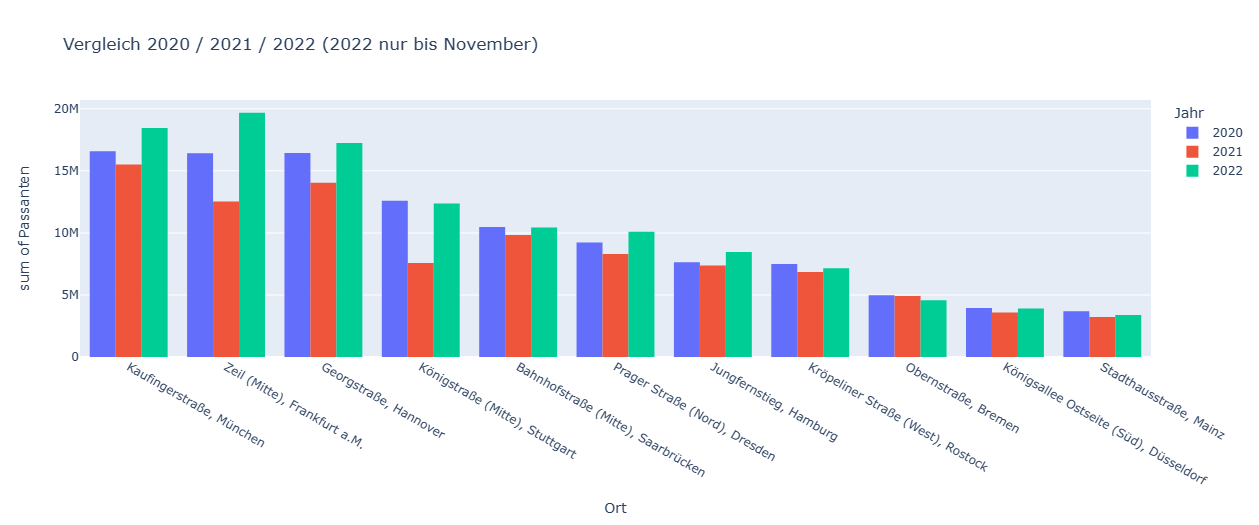
\includegraphics[width=\linewidth]{images/absJahresvergleich.png}
    \caption{Vergleich der Standorte für die einzelnen Jahre}
    \label{fig:absJahresvergleich}
\end{figure}

\subsection{Uhrzeitenvergleich}
Vor allem für Ladenbesitzer ist es nicht nur wichtig zu wissen, an welchem Wochentag die meisten Menschen an den jeweiligen Standorten unterwegs sind, sondern auch um welche Uhrzeit. 
Betrachtet werden hier alle Standorte gleichzeitig, um ein allgemeines Gefühl zu erhalten, welche Uhrzeiten besonders beliebt sind. Möchte man nur einen speziellen Standort betrachten, muss man die Eingabedaten zuvor nur auf den jeweiligen Standort filtern und die Funktion erzielt die gleichen Ergebnisse. In SQL übersetzt würde die Funktion folgendens berechnen, $ SUM(pedestrians) GROUP BY Month, Hour $, betrachtet also für alle Standorte gleichzeitig wie viele Passanten pro Monat pro jeweiliger Stunde gemessen wurde:

\bigbreak
\begin{tcolorbox}[breakable, size=fbox, boxrule=1pt, pad at break*=1mm,colback=cellbackground, colframe=cellborder]
\prompt{In}{incolor}{2}{\boxspacing}
\begin{Verbatim}[commandchars=\\\{\}]
\PY{k}{def} \PY{n+nf}{absPerHour}\PY{p}{(}\PY{n}{data}\PY{p}{,} \PY{n}{years}\PY{p}{)}\PY{p}{:}
  \PY{n}{dataTime} \PY{o}{=} \PY{n}{data}\PY{o}{.}\PY{n}{loc}\PY{p}{[}\PY{n}{data}\PY{p}{[}\PY{l+s+s1}{\PYZsq{}}\PY{l+s+s1}{year}\PY{l+s+s1}{\PYZsq{}}\PY{p}{]}\PY{o}{.}\PY{n}{isin}\PY{p}{(}\PY{n}{years}\PY{p}{)}\PY{p}{]}
  \PY{n}{dataTL} \PY{o}{=} \PY{n+nb}{list}\PY{p}{(}\PY{p}{)}
  \PY{n}{monate} \PY{o}{=} \PY{p}{[}\PY{l+s+s2}{\PYZdq{}}\PY{l+s+s2}{Januar}\PY{l+s+s2}{\PYZdq{}}\PY{p}{,} \PY{l+s+s2}{\PYZdq{}}\PY{l+s+s2}{Februar}\PY{l+s+s2}{\PYZdq{}}\PY{p}{,} \PY{l+s+s2}{\PYZdq{}}\PY{l+s+s2}{März}\PY{l+s+s2}{\PYZdq{}}\PY{p}{,} \PY{l+s+s2}{\PYZdq{}}\PY{l+s+s2}{April}\PY{l+s+s2}{\PYZdq{}}\PY{p}{,} \PY{l+s+s2}{\PYZdq{}}\PY{l+s+s2}{...}\PY{l+s+s2}{"}{]}
  \PY{n}{df} \PY{o}{=} \PY{n}{pd}\PY{o}{.}\PY{n}{DataFrame}\PY{p}{(}\PY{n}{columns}\PY{o}{=}\PY{p}{[}\PY{l+s+s2}{\PYZdq{}}\PY{l+s+s2}{Monat}\PY{l+s+s2}{\PYZdq{}}\PY{p}{,} \PY{l+s+s2}{\PYZdq{}}\PY{l+s+s2}{Stunde}\PY{l+s+s2}{\PYZdq{}}\PY{p}{,} \PY{l+s+s2}{\PYZdq{}}\PY{l+s+s2}{Passanten}\PY{l+s+s2}{\PYZdq{}}\PY{p}{]}\PY{p}{)}
  \PY{k}{for} \PY{n}{month} \PY{o+ow}{in} \PY{n+nb}{range}\PY{p}{(}\PY{l+m+mi}{12}\PY{p}{)}\PY{p}{:}
    \PY{n}{tmp} \PY{o}{=} \PY{n}{dataTime}\PY{o}{.}\PY{n}{loc}\PY{p}{[}\PY{n}{dataTime}\PY{p}{[}\PY{l+s+s1}{\PYZsq{}}\PY{l+s+s1}{month}\PY{l+s+s1}{\PYZsq{}}\PY{p}{]} \PY{o}{==} \PY{p}{(}\PY{n}{month} \PY{o}{+} \PY{l+m+mi}{1}\PY{p}{)}\PY{p}{]}
    \PY{n}{tsum} \PY{o}{=} \PY{n}{tmp}\PY{o}{.}\PY{n}{groupby}\PY{p}{(}\PY{l+s+s1}{\PYZsq{}}\PY{l+s+s1}{hour}\PY{l+s+s1}{\PYZsq{}}\PY{p}{)}\PY{p}{[}\PY{l+s+s1}{\PYZsq{}}\PY{l+s+s1}{pedestrians}\PY{l+s+s1}{\PYZsq{}}\PY{p}{]}\PY{o}{.}\PY{n}{sum}\PY{p}{(}\PY{p}{)}
    \PY{k}{for} \PY{n}{hour} \PY{o+ow}{in} \PY{n+nb}{range}\PY{p}{(}\PY{l+m+mi}{0}\PY{p}{,} \PY{l+m+mi}{24}\PY{p}{)}\PY{p}{:}
      \PY{n}{df} \PY{o}{=} \PY{n}{df}\PY{o}{.}\PY{n}{append}\PY{p}{(}\PY{p}{\PYZob{}}\PY{l+s+s2}{\PYZdq{}}\PY{l+s+s2}{Monat}\PY{l+s+s2}{\PYZdq{}} \PY{p}{:} \PY{n}{monate}\PY{p}{[}\PY{n}{month}\PY{p}{]}\PY{p}{,} \PY{l+s+s2}{\PYZdq{}}\PY{l+s+s2}{Stunde}\PY{l+s+s2}{\PYZdq{}} \PY{p}{:} \PY{n}{hour}\PY{p}{,} \PY{l+s+s2}{\PYZdq{}}\PY{l+s+s2}{Passanten}\PY{l+s+s2}{\PYZdq{}} \PY{p}{:} \PY{n}{tsum}\PY{o}{.}\PY{n}{iloc}\PY{p}{[}\PY{n}{hour}\PY{p}{]} \PY{p}{\PYZcb{}}\PY{p}{,} \PY{n}{ignore\PYZus{}index}\PY{o}{=}\PY{k+kc}{True}\PY{p}{)}
  \PY{k}{return} \PY{n}{df}
\PY{n}{absHours} \PY{o}{=} \PY{n}{absPerHour}\PY{p}{(}\PY{n}{data}\PY{p}{,} \PY{p}{[}\PY{l+m+mi}{2020}\PY{p}{]}\PY{p}{)}
\end{Verbatim}
\end{tcolorbox}
\bigbreak

Das resultierende Pandas-Dataframe kann anschließend wieder mit Plotly und dessen Linien-Plot visualisiert werden. Zu erkennen ist, dass der Höhepunkt, unabhängig des Monats gegen ca. 16 Uhr erreicht wird. 

\begin{figure}[h!]
    \vspace{0.2cm}
    \centering
    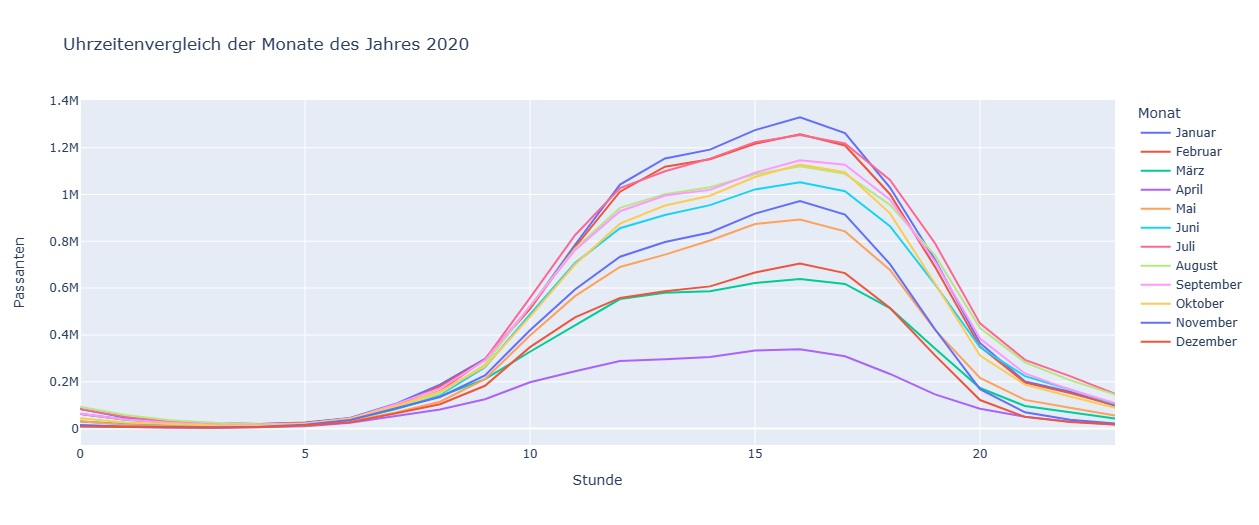
\includegraphics[width=\linewidth]{images/absHour.png}
    \caption{Vergleich der Passantenanzahl pro Monat pro Stunde}
    \label{fig:absStundenvergleich}
\end{figure}